\documentclass[12pt,a4paper]{article}
\usepackage{preamble}


\PassOptionsToPackage{
  backend=biber,
  style=numeric, % eller authoryear
  sorting=nyt,
  giveninits=true,
  maxbibnames=99,
  doi=false,isbn=false,url=true,
  dashed=false
}{biblatex}


\usepackage{preamble}
\usepackage{xcolor}
\usepackage{booktabs}
\usepackage{circuitikz}
\usepackage{float} % for [H] exact figure placement
\usetikzlibrary{arrows.meta}

\usepackage{pgfplots}
\pgfplotsset{compat=1.18}

\usepackage{amsmath}




\addbibresource{./referanser.bib}

% ------ Metadata ------
\newcommand{\institution}{FHS/Cyberingeniørskolen}
\newcommand{\laboratory}{Elektronikklaboratoriet}
\newcommand{\coursecode}{ING2508 \; Kretsteknikk}
\newcommand{\assignmentno}{V04}
\newcommand{\assignmenttype}{MÅLJOURNAL}
\newcommand{\assignmenttitle}{TRANSISTOR FORSTERKINGKOBLINGER}
\newcommand{\studentname}{Tor Johan Aleksandersen}
\newcommand{\partnername}{Morten Cleveland}
\newcommand{\class}{VING 78}
\newcommand{\labdate}{23. april 2026}
\newcommand{\submissiondate}{\today}

\begin{document}

\input{frontpage}

\pagenumbering{arabic}
\setcounter{page}{1}

\section{Innledning}
I dette forsøket studeres en transistorbasert FE-forsterker (felles emitter) med fokus på hvordan kretsens oppbygning påvirker signalforsterkning og signalform. Ved hjelp av både teoretiske beregninger og praktiske målinger analyseres sammenhengen mellom inngangssignal og utgangssignal, samt hvordan arbeidspunktet påvirker forsterkerens oppførsel.
\\[1em]
Det legges særlig vekt på å undersøke spenningsforsterkning, faseforskyvning og fenomener som klipping og ikke-lineær respons. Videre studeres hvordan endringer i komponentverdier, spesielt kollektormotstanden, påvirker forsterkningen.
\\[1em]
Etter gjennomført forsøk skal vi ha god kjennskap til FE-forsterkere, samt forstå sentrale begreper som spenningsforsterkning, faseforskyvning, inngangsimpedans og utgangsimpedans.
\clearpage

\section{Instrument- og komponentliste}

\subsection{Instrumentliste}
\begin{table}[h]
    \centering
    \caption{Instrumentliste}
    \vspace{1em}
    \label{tab:instrumentliste}
    \begin{tabular}{|l|l|l|c|}
        \hline
        \rowcolor[gray]{0.9}
        \textbf{Instrument} & \textbf{Beskrivelse} & \textbf{Serie Nr.} & \textbf{Antall} \\ \hline

        Signalgenerator & SFG-2401 & 924925 \\ \hline
        Spenningsforsyning & GWINSTEK GPS-3030 & 834968 \\ \hline
        Digitalt Multimeter & FLUKE-8808A & 2097019 \\ \hline
        Digitalt Multimeter & FLUKE-8808A & 2105052 \\ \hline
        Oscilloskop & GDS-1104B & GEX821030 \\ \hline

    \end{tabular}
\end{table}

\subsection{Komponentliste}
\begin{table}[h]
    \centering
    \caption{Komponentliste}
    \vspace{1em}
    \label{tab:komponentliste}
    \begin{tabular}{|l|l|c|}
        \hline
        \rowcolor[gray]{0.9}
        \textbf{Komponenttype} & \textbf{Verdi} & \textbf{Antall} \\ \hline
        Motstand & 1k$\Omega$ & 1 \\ \hline
        Motstand & 1.2k$\Omega$ & 2 \\ \hline
        Motstand & 5.6k$\Omega$ & 1 \\ \hline
        Motstand & 10k$\Omega$ & 1 \\ \hline
        Motstand & 22k$\Omega$ & 2 \\ \hline
        Motstand & 82k$\Omega$ & 1 \\ \hline
        Motstand & 1M$\Omega$ & 1 \\ \hline
        Dekademotstand & 3.9k$\Omega$ & 1 \\ \hline
        Kondensator & 10$\mathrm{\mu}$F & 2 \\ \hline
        Kondensator & 47$\mathrm{\mu}$F & 1 \\ \hline
        Transistor & BC546B & 1 \\ \hline
        Koblingsbrett & & 1 \\ \hline
    \end{tabular}
\end{table}

\clearpage

\section{Teori}






\subsection{Forsterkerkretsen}
Dette er forsterkerkretsen vi skal studere, gjøre beregninger på og legge et teoretisk grunnlag for forsterkerkretser.

\begin{figure}[H]
\centering
\begin{circuitikz}[american]
    % Transistor
    \draw (6,0) node[npn, tr circle] (Q1) {$Q_1$};

    % Input capacitor and input label
    \draw (0,0) node[left] {$V_i$}
        to[C, a=$10\mu\mathrm{F}$, l=$C_4$] (3,0)
        -- (Q1.B);

    % Bias resistors
    \draw (3,0) to[R, l_=$R_6\,\,22\mathrm{k}\Omega$] ++(0,-3) node[ground]{};
    \draw (3,0) -- ++(0,1.5) coordinate (Btop);
    \draw (Btop) to[R, l=$R_4\,\,82\mathrm{k}\Omega$] ++(0,3) coordinate (VCC);

    % Collector resistor
    \draw (Q1.C) to[R, l=$R_2\,\,5.6\mathrm{k}\Omega$] (Q1.C |- VCC);

    % Connect top rail
    \draw (VCC) -- (Q1.C |- VCC) -- ++(4,0)
        to[battery1, a=$V_1$, v^>=$18\mathrm{V}$] ++(0,-2) node[ground]{};

    % Emitter resistor
    \draw (Q1.E) to[R, l=$R_3\,\,1.2\mathrm{k}\Omega$] ++(0,-2.5) node[ground]{};

    % Output capacitor and output label
    \draw (Q1.C)
        to[C, a=$10\mu\mathrm{F}$, l=$C_5$] ++(4,0)
        node[right] {$V_0$};

    % Optional transistor type text
    \node[above] at (5, 0.5) {BC546B};

\end{circuitikz}
\caption{Transistorkobling.}
\label{fig:transistorkretsen}
\end{figure}

\noindent
Tar vi for oss koblingen kan vi analysere den og se på effekten av endringer. Hvis base-emitterspenningen øker, leder transistoren mer og basestrømmen øker kraftig. Dersom kollektorstrømmen endres, kan vi se at kollektorstrømmen må synke pågrunn av et større spenningsfall over $R_2$. $I_E$ øker med $I_C$ proporsjonalt og $V_E$ vil dermed øke pågrunn av større spenningsfall over emittermotstanden. Dersom $V_{BE}$ og $I_B$ synker, vil effekten reverseres.
\\[1em]
Fra databladet kan vi leser vi $\beta = 290$.

\begin{table}[H]
\centering
\caption{Sammenheng mellom spenninger og strømmer i transistoren.}
\label{tab:transistor_sammenheng}
\vspace{1em}
\begin{tabular}{lc}
\toprule
\textbf{Endring} & \textbf{Effekt} \\
\midrule
$\uparrow V_{BE}$ & $\uparrow I_C$ \\
$\downarrow V_{BE}$ & $\downarrow I_C$ \\
\midrule
$\uparrow I_C$ & $\downarrow V_C$ \\
$\downarrow I_C$ & $\uparrow V_C$ \\
\midrule
$\uparrow I_C$ & $\uparrow V_E$ \\
$\downarrow I_C$ & $\downarrow V_E$ \\
\midrule
$\uparrow I_C$ & $\downarrow V_{CE}$ \\
$\downarrow I_C$ & $\uparrow V_{CE}$ \\
\bottomrule
\end{tabular}
\end{table}

\noindent
Vi skal finne signalforsterkingen for følgende verdier av $R_2$: 
$4.7\,\text{k}\Omega$, $5.6\,\text{k}\Omega$ og $6.8\,\text{k}\Omega$.

\begin{figure}[H]
\centering
\begin{circuitikz}[american]

% Spenningskilde
\draw (0,4) to[battery1, v^>=$V_1$] (0,0);

% Toppnode
\draw (0,4) -- (3,4);

% R4
\draw (3,4) to[R, l=$R_4\,82\,\text{k}\Omega$] (3,2);

% Node til base
\draw (3,2) -- (5,2) node[right] {Base};

% R6 til jord
\draw (3,2) to[R, l=$R_6\,22\,\text{k}\Omega$] (3,0);

% Jord
\draw (0,0) -- (3,0) node[ground]{};

\end{circuitikz}
\caption{Basekrets før Thevenin-transformasjon.}
\end{figure}

\noindent
Vi transformerer først basekretsen til sin Thevenin-ekvivalent.

\begin{gather*}
V_{\text{th}} = V_1 \cdot \frac{R_6}{R_6 + R_4} \\
V_{\text{th}} = 18\,\text{V} \cdot \frac{22\,\text{k}\Omega}{22\,\text{k}\Omega + 82\,\text{k}\Omega} \\
V_{\text{th}} = 3.81\,\text{V}
\end{gather*}

\begin{gather*}
R_{\text{th}} = R_4 \parallel R_6 \\
R_{\text{th}} = \frac{R_4 \cdot R_6}{R_4 + R_6} \\
R_{\text{th}} = \frac{82\,\text{k}\Omega \cdot 22\,\text{k}\Omega}{82\,\text{k}\Omega + 22\,\text{k}\Omega} \\
R_{\text{th}} = 17.3\,\text{k}\Omega
\end{gather*}



\noindent
Vi kan nå regne for basestrømmen og $r_e$.
\begin{gather*}
I_B = \frac{V_{th} - V_{BE}}{R_{th} + \left(\beta + 1\right) R_3} \\
I_B = \frac{3.808\text{V} - 0.7\text{V}}{17.3\text{k}\Omega + \left(290 + 1\right) 1.2\text{k}\Omega} \\
I_B = 8.46 \mu \text{A}
\end{gather*}

\begin{gather*}
r_e = \frac{V_T}{I_E} = \frac{V_T}{\left(\beta + 1\right) I_B} \\
r_e = \frac{26\text{mA}}{\left(290 + 1\right) 8.46 \mu \text{A}} \\
r_e = 10.56 \Omega
\end{gather*}

\noindent
For å regne signalforsterkingen må vi analysere kretsen i sin AC-state. Kretsen under er omgjort fra figur~\ref{fig:transistorkretsen} i sin AC-state. Kondensatorer og kilder er kortsluttet og transistoren er omgjort.

\begin{figure}[H]
\centering
\begin{circuitikz}[american]

% Top signal line
\draw (0,0) node[left] {$V_i$} -- (5.6,0);
\draw (8,0) -- (13.6,0) node[right] {$V_o$};

% Left shunt resistors
\draw (1.4,0) to[R, l=$R_4$] (1.4,-3) node[ground]{};
\draw (3.5,0) to[R, l=$R_6$] (3.5,-3) node[ground]{};

% Middle connection (shifted)
\draw (5.6,-3) -- (8,-3);

% Beta*re resistor
\draw (5.6,0) to[R, l=$\beta r_e$] (5.6,-3);

% Emitter resistor
\draw (6.8,-3) to[R, l=$R_3$] (6.8,-6) node[ground]{};

% Controlled current source (shifted)
\draw (8,0) to[cI, l=$\beta I_B$] (8,-3);

% Output resistors (shifted)
\draw (10.1,0) to[R, l=$r_o$] (10.1,-3) node[ground]{};
\draw (11.5,0) to[R, l=$R_2$] (11.5,-3) node[ground]{};

\end{circuitikz}
\caption{AC-ekvivalent krets for transistorforsterkeren.}
\label{fig:ac-ekvivalent}
\end{figure}

\noindent
\begin{gather*}
A_v = \frac{V_o}{V_i} \\
A_v = - \frac{I_{R2}R_2}{I_B\cdot\beta r_e + I_E R_3} \\
A_v = - \frac{\beta I_B R_2}{I_B\cdot\beta r_e + I_B \left(\beta + 1\right) R_3}, \qquad \beta + 1 \approx \beta \\
A_v \approx - \frac{R_2}{r_e + R_3}
\end{gather*}
\vspace{1em}
\[
A_v = - \frac{R_2}{1200\Omega + 10.56\Omega}
\]







\begin{table}[H]
\centering
\caption{Resultater for gain $A_v$.}
\label{tab:gain_utregnet}
\vspace{1em}
\begin{tabular}{lc}
\toprule
\textbf{$R_c$} & \textbf{$A_v$} \\
\midrule
$4.7\,\text{k}\Omega$ & -3.88 \\
$5.6\,\text{k}\Omega$ & -4.59 \\
$6.8\,\text{k}\Omega$ & -5.57 \\
\bottomrule
\end{tabular}
\end{table}

\noindent
Faseforskyvingen mellom basis og kollektor kan leses gjennom gain $A_v$. Denne er negativ, noe som viser $180\degree$ faseforskyving. Dette kan også leses av kretsen, dersom inngangsspenningen øker, øker strømmen. Ved høyere strøm øker spenningsfallet over kollektorresistansen og utgangsspenningen synker. Dermed vil utgangsspenningen synke når inngangsspenningen øker, derav $180\degree$ faseskift. Kondensatorene $C_4$ og $C_5$ har som hensikt å fjerne DC-komponenten fra det eksterne signalet. Dersom vi avkobler emittermotstanden $R_3$ med en kondensator, vil kretsen være uendret i DC-analyse, men i AC-analyse ser vi en helt annen krets. Siden kondensatoren blir kortsluttet, vil da gainen gis ved:
\[
A_v = - \frac{R_2}{r_e} = - \frac{R_2}{10.56\Omega}
\]

\begin{table}[H]
\centering
\caption{Resultater for gain $A_v$ ved avkoblet emittermotstand.}
\label{tab:gain_utregnet_avkoblet_emitter}
\vspace{1em}
\begin{tabular}{lc}
\toprule
\textbf{$R_c$} & \textbf{$A_v$} \\
\midrule
$4.7\,\text{k}\Omega$ & -445.1 \\
$5.6\,\text{k}\Omega$ & -530.3 \\
$6.8\,\text{k}\Omega$ & -644.0 \\
\bottomrule
\end{tabular}
\end{table}

\subsubsection{Arbeidslinjen}
KVL i kollektordelen av forsterken kan uttrykkes:
\begin{gather*}
    V_CC = I_C R_C + V_{CE} + I_E R_E, \quad I_E \approx I_C \\
    V_1 = I_C R_2 + V_{CE} + I_C R_3 \\
    18\text{V} = I_C \left(5.6\text{k}\Omega + 1.2\text{k}\Omega\right) + V_{CE} \\
    18\text{V} = I_C \left(6.8\text{k}\Omega \right) + V_{CE}
\end{gather*}

\noindent
Nå har vi to ukjente og kan lage arbeidslinjen for denne forsterkeren.

\begin{gather*}
    I_C = 0\text{mA} \rightarrow V_{CE} = 18\text{V} \\
    V_{CE} = 0\text{V} \rightarrow I_C = 2.65\text{mA}
\end{gather*}

\noindent
Arbeidslinjen er lineær og kan dras fra disse to punktene.

\begin{figure}[H]
\centering
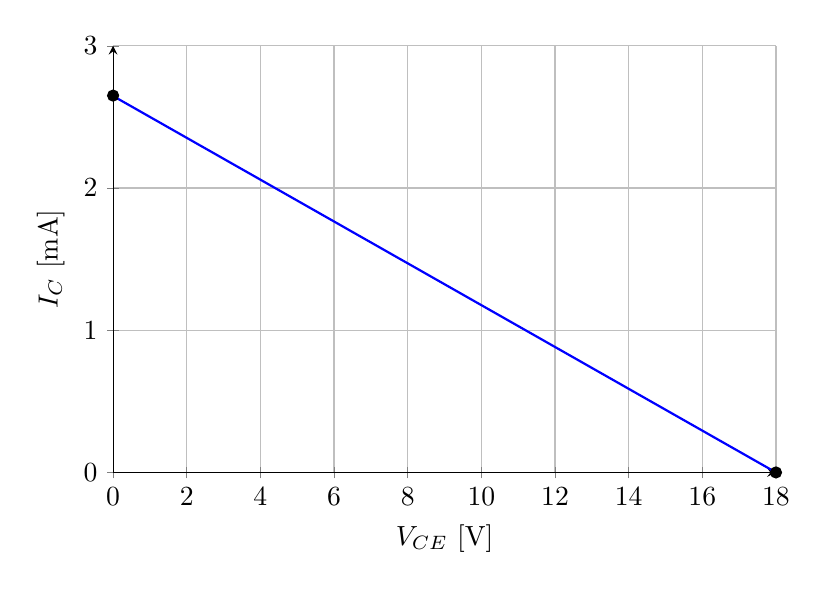
\begin{tikzpicture}
\begin{axis}[
    width=10cm,
    height=7cm,
    xlabel={$V_{CE}$ [V]},
    ylabel={$I_C$ [mA]},
    xmin=0, xmax=18,
    ymin=0, ymax=3,
    grid=both,
    axis lines=left,
    domain=0:18,
    samples=100,
]

% Lastlinje: I_C = (18 - V_CE)/6.8k
\addplot[thick, blue] { (18 - x)/6.8 };

% Punkter
\addplot[only marks, mark=*] coordinates {(18,0) (0,2.65)};

% Labels på punktene
\node at (axis cs:18,0) [anchor=north west] {$(18,0)$};
\node at (axis cs:0,2.65) [anchor=south east] {$(0,2.65)$};

\end{axis}
\end{tikzpicture}
\caption{Arbeidslinje for transistorforsterkeren}
\end{figure}
\clearpage

\section{Gjennomføring med måleresultater}

\subsection{FE-forsterker med emittermotstand}

\subsubsection{Krets 1 - forsterking/faseforskyving}

\subsubsection{Krets 2 - kollektormotstandens innvirkning}

\subsubsection{Krets 3 - Inngangsimpedans}

\subsubsection{Krets 4 - Utgangsimpedans}

\subsection{FE-forsterker med avkoblet emittermotstand}


\clearpage

\input{sections/diskusjon}
\clearpage

\end{document}
